\chapter{Evaluation of Distributed MCTS Algorithms}

\todo{Úvod ke kapitole, co tu bude atd..}

\section{Ms Pac-Man vs Ghosts Framework}

For the purposes of evaluation of algorithms proposed in Chapter \ref{chap_dmcts_design}, we
have chosen the Ms Pac-Man vs Ghosts Framework (\ref{PacmanVsGhosts}) which is easy-to-use
framework allowing implementation of players for well-known old game Pac-Man in Java. Here we
will extract basics of the game rules used in the framework and afterwards we will
describe modifications of the rules we have done and reasons for them.

Ms Pac-Man is a game played in a maze in which two sides compete, the Pac-Man and four ghosts.
There are pills everywhere in the maze and Pac-Mans purpuse is to gather all the pills, each
for 10 points. Once all the pills are eaten, the game continues in a next maze. To complicate
the life of Pac-Man, ghosts are moving around the maze pursuing the Pac-Man and trying to
minimize its score. If the Pac-Man is caught, it will lose one life and if has any life
remaining, starts again from its starting position. Pills remain eaten after the life loss.
Ghosts appear in so-called lair at the beginning of each round and after Pac-Man's life loss
from where they start after a several time (different for each ghost). Beside regular pills,
each maze contains four power pills which are awarded with 50 points and when eaten by Pac-Man,
ghosts become edible and twice slower for certain period of time. Pac-Man can eat ghosts during 
this period for
reward of 200 points for first eaten ghost and 400, 800 and 1600 points for other ghosts.
Eaten ghost starts in lair again.

Exact rules of the Ms Pac-Man vs Ghosts game can be found on the project webpage. The game was
additionally modified for purposes of testing of our algorithms. Biggest change of rules is
removing power pills from the mazes together with entire edible ghosts mechanism. Reason for
this decision is lowering the variability of results. When Pac-Man is pursuing edible ghosts,
there is big difference in score when it eats different number of ghosts. For the same reason
three more modification have been done. Pac-Man has only one life, game ends after the first
maze is cleared and random ghosts' reversal is suppressed what is a rule
which adds stochasticity to the game. If the rule is on, there is a 0.15\% probability each tick of
a game that all
ghosts accidentally change their direction. \todo{max. délka hry}
An example of a situation from the game without
power pills is depicted by Figure \ref{fig_pacman_framework}.

\begin{figure}
\begin{center}
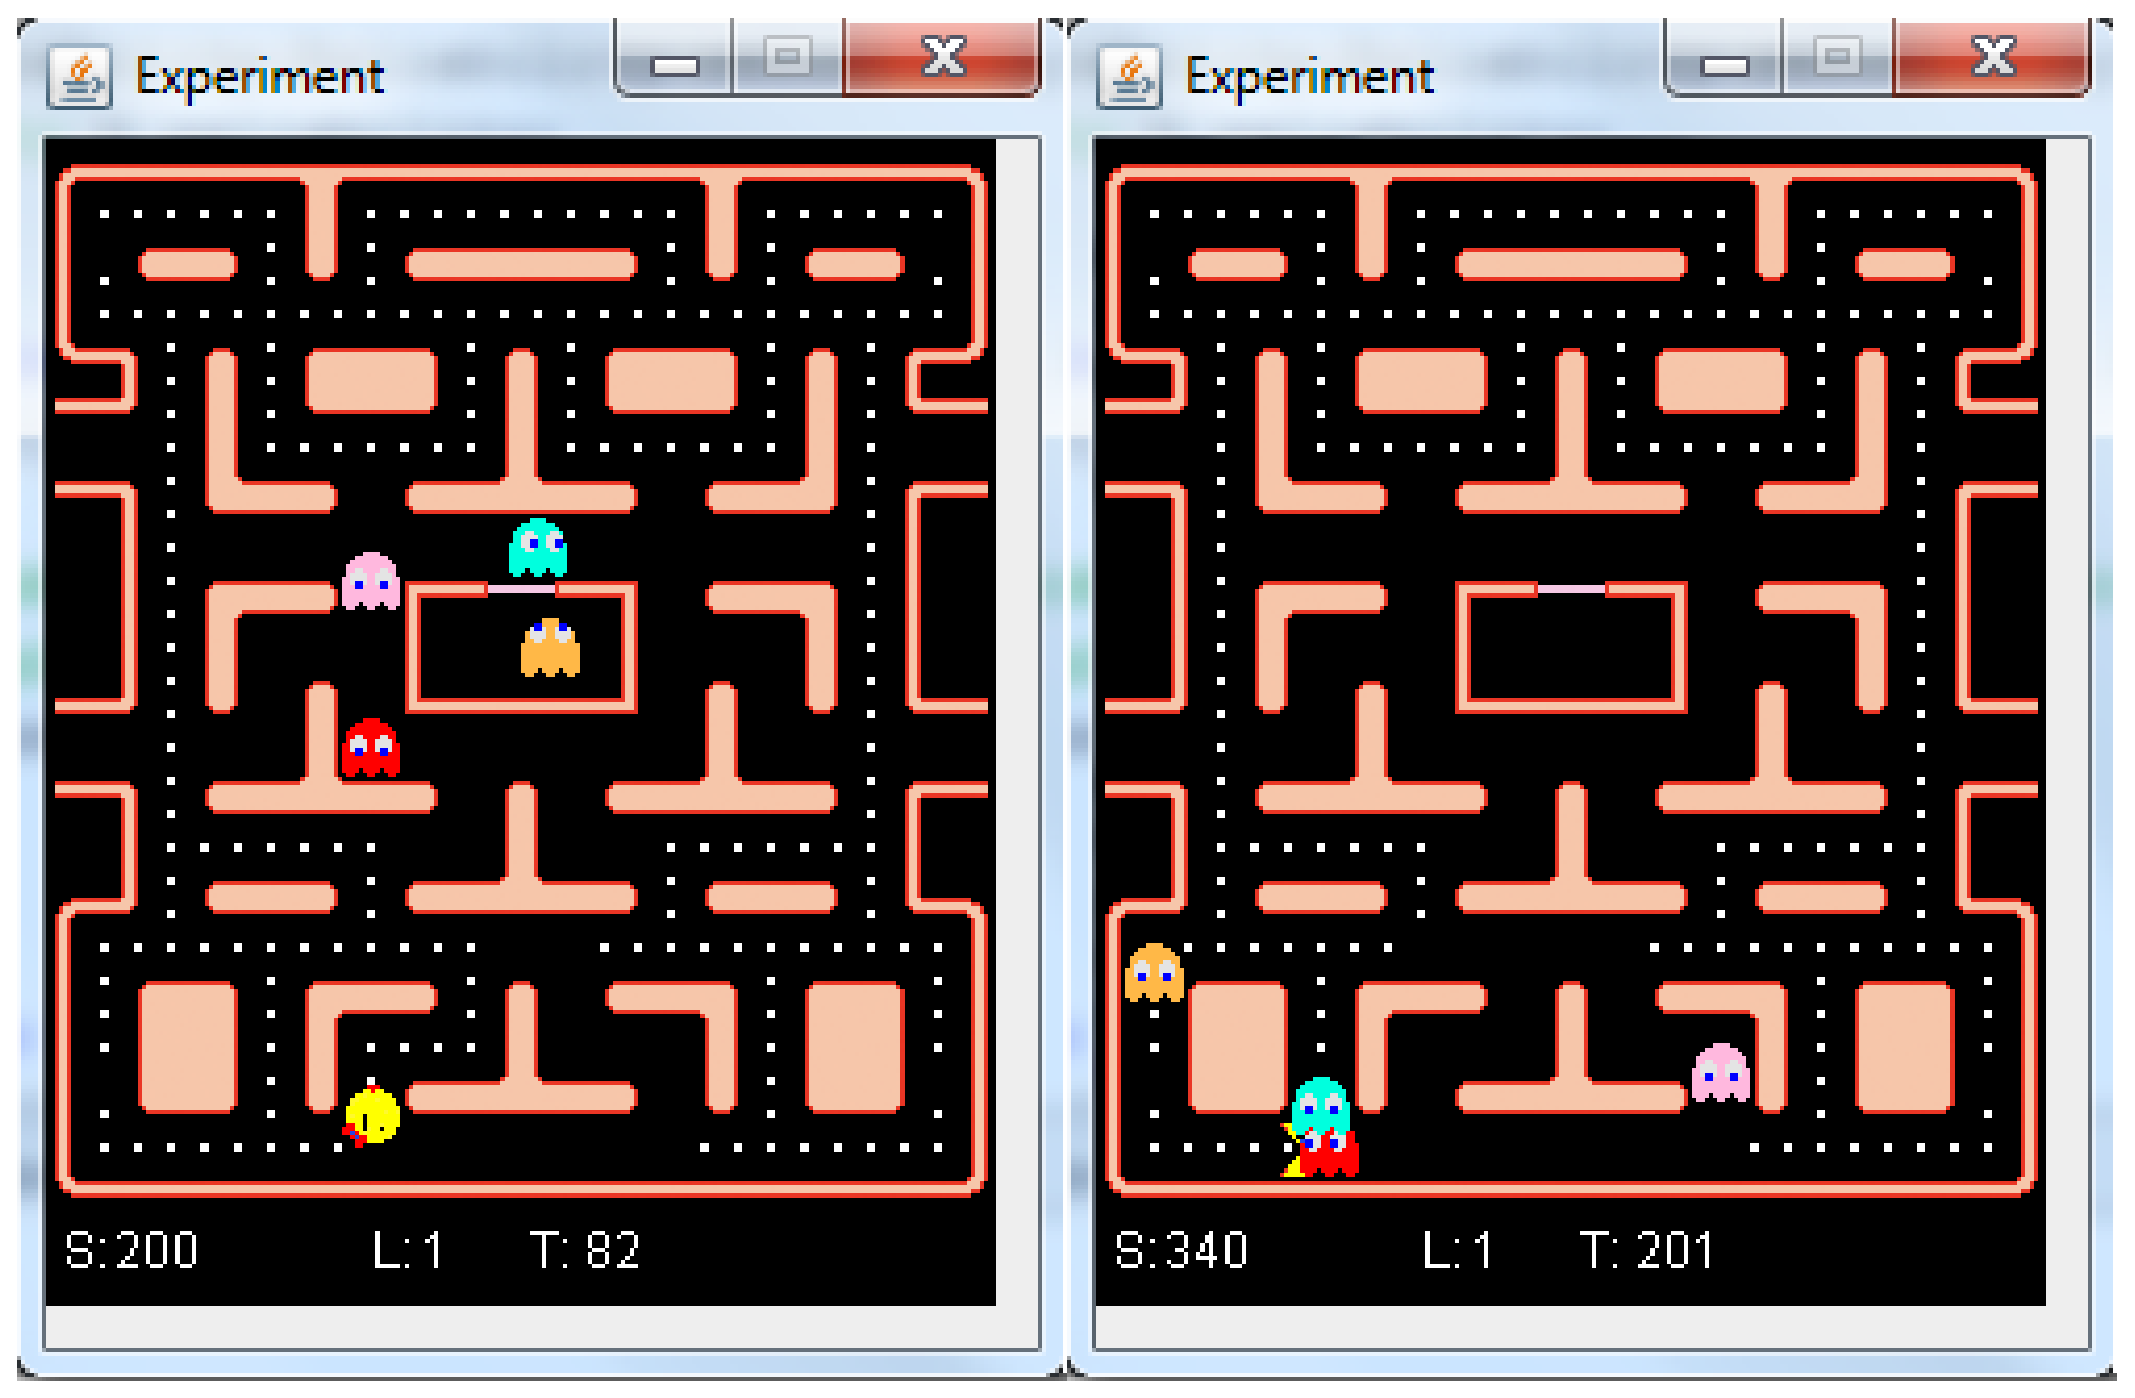
\includegraphics[width=14cm]{img/pacman_framework.eps}
\end{center}
\caption{\footnotesize Game of Ms Pacman.}{\footnotesize Left picture shows the game few moments after it began. Three
ghosts started to hunt the Pac-Man while the orange one is still waiting in lair. Right
picture, on the other hand, shows the game just before the end. Pac-Man does not have any
escape path and is being caught with in a while with no life remaining.}
\label{fig_pacman_framework}
\end{figure}

Pac-Man has the same movement speed as non-edible ghosts. Maze is divided into small 


\section{Implementation Notes}

\section{Methodics}

\section{MCTS Tuning}

\section{Comparison of the Algorithms}

\section{Conclusion}
